\documentclass{standalone}
\usepackage{tikz}
\usepackage{ctex,siunitx}
\usepackage{tkz-euclide}
\usepackage{amsmath}
\usetikzlibrary{patterns, calc}
\usetikzlibrary {decorations.pathmorphing, decorations.pathreplacing, decorations.shapes,}
\begin{document}
\small
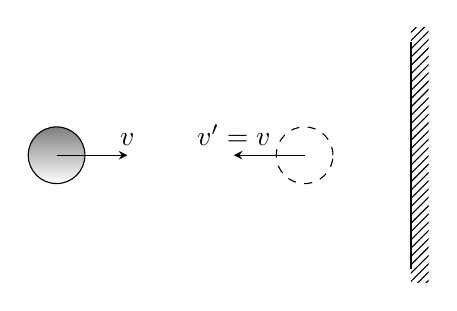
\begin{tikzpicture}[>=stealth,scale=0.9]
  \draw [thick](5,1.6)--(5,-1.6);
  \fill [pattern=north east lines](5,-1.8) rectangle(5.25,1.8);
  \draw [shade](0,0) circle (4mm);
  \draw [dashed] (3.5,0) circle (4mm);
  \draw[->](0,0)--(1,0) node [above]{$v$};
  \draw[->](3.5,0)--(2.5,0)node [above]{$v'=v$};
\end{tikzpicture}
\end{document}